\paragraph{Observations, actions, reward.}
The observation is an egocentric $21\times21$ crop of the tile map, one-hot
over nine tile types, plus five scalars: the facing direction as a one-hot of
four and the elapsed fraction of the step budget. The action space is
\texttt{Discrete(6)}: four moves, \textsc{build} and \textsc{mine}. The reward
is
\begin{equation}
r_t \;=\; -0.01 \;+\; 0.015\,(d_{t-1}-d_t) \;+\; 3\cdot\mathbf{1}[\text{correct flag}],
\label{eq:reward}
\end{equation}
where $d_t$ is the cost-to-go in cells to the nearest rewarding flag. The
middle term is potential-based shaping \citep{ng1999shaping} in its
undiscounted form, so pacing back and forth nets nothing. Episodes end at any
flag or after $800$ steps; the discount is $\gamma=0.99$.

\paragraph{Generation, step by step.}
Every map is a deterministic function of an integer seed and a category.
Figure~\ref{fig:mapgen} shows the six stages on one real map; the parameters
are collected in Table~\ref{tab:mapgen}.
\begin{enumerate}[leftmargin=1.4em, itemsep=1pt]
\item \textbf{Heightmap.} A five-octave OpenSimplex field
\citep{spencer2014opensimplex} on the $32\times64$ grid, octave $k$ at
wavelength $\lambda_0/2^k$ with weight $2^{-k}$, normalised by the weight sum.
\item \textbf{Domain warp.} Two independent two-octave fields displace the
sampling coordinates by up to $0.10\max(H,W)$ cells, so lakes and massifs get
irregular coastlines instead of blobs.
\item \textbf{Overlays.} Two to four lakes are carved and two to four
mountains raised, each a round logistic disk or an irregular massif of three to
five Gaussian lobes with equal probability, and at most one meandering ridge is
added. Radii are drawn small-biased, $R = \max(H,W)\,(0.02 + 0.075\,u^2)$ with
$u\sim\mathcal{U}(0,1)$.
\item \textbf{Quantile threshold.} Cells below the $w$-quantile of the field
become water and cells above the $(1-r)$-quantile become rock, so every map hits
its category's water and rock fractions $(w,r)$ exactly: lakes $(0.245,
0.035)$, rocky $(0.035, 0.245)$, balanced $(0.14, 0.14)$. Sand and dirt
speckles are added on a fraction of the one-cell ring around water and rock;
both are walkable and only cosmetic.
\item \textbf{Bands, trees, corridor.} The ten leftmost and rightmost columns
are cleared; the agent spawns at the middle of the left edge. About $3\%$ of
cells become impassable tree patches of radius one or two, placed with a strong
bias toward the top and bottom rows so that hugging the top or bottom edge is not a free route;
patches are removed, last placed first, until the flags are reachable with
trees as the only barrier. The sixteen columns before the passage are then reset
to grass: the memory corridor.
\item \textbf{Passage and flags.} A line of trees one column from the right
edge, open only at a three-cell passage at the middle rows, and two single-cell flags on the right
edge at one quarter and three quarters of the height. The rewarding flag is the
bottom one when $w > 1.5\,r$, the top one when $r > 1.5\,w$, and either
otherwise.
\item \textbf{Winnability guard.} A breadth-first search from the spawn to the
rewarding flag treating the category's crossable tile as passable (water for
lakes, rock for rocky, each in turn for balanced) must succeed; otherwise the
seed is advanced by a large prime and the map regenerated, up to $400$ times.
\end{enumerate}

\begin{figure}[t]
\centering
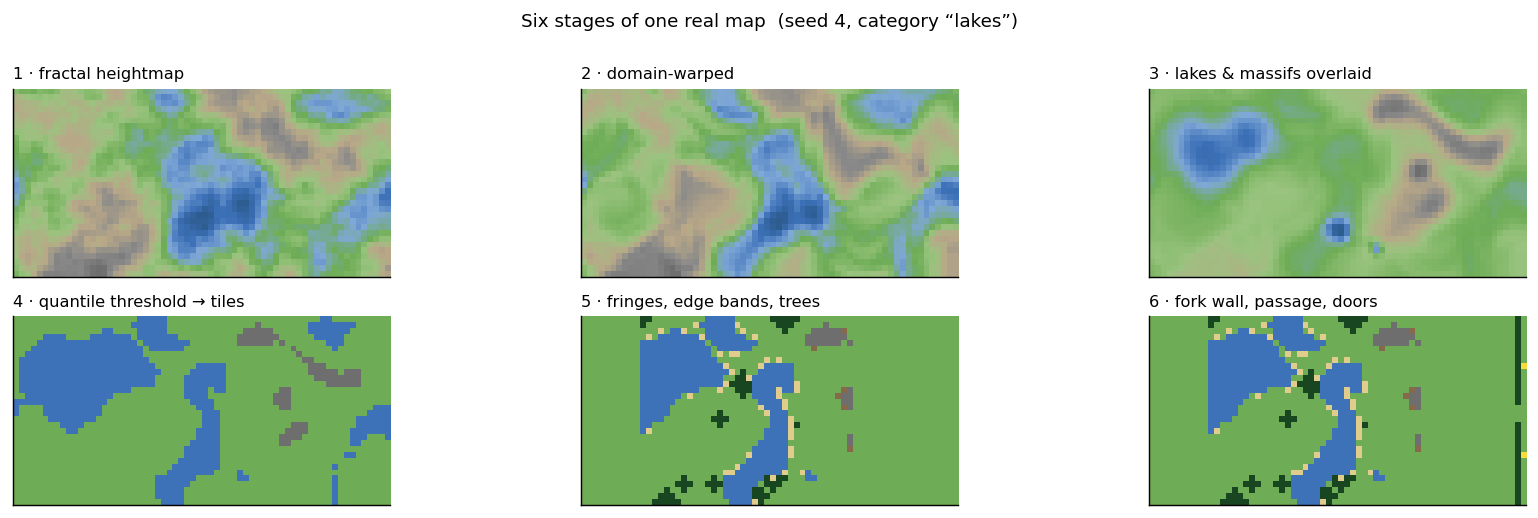
\includegraphics[width=\linewidth]{figures/mapgen_pipeline.png}
\caption{\textbf{One map, six stages.} Fractal heightmap, domain warp, overlaid
lakes and massifs, quantile threshold to tiles, cosmetic fringes with edge bands
and tree patches, and finally the passage and flags. The example is a
lakes map; a rocky map differs only in the two quantiles of step~4.}
\label{fig:mapgen}
\end{figure}

\begin{table}[t]
\centering
\footnotesize
\caption{\textbf{Map-generation parameters.} $H\times W = 32\times64$;
$\max(H,W)=64$. Uniform integer ranges are inclusive.}
\label{tab:mapgen}
\begin{tabular}{@{}p{3.0cm}p{4.5cm}p{5.5cm}@{}}
\toprule
Parameter & Value & Meaning \\
\midrule
Base wavelength $\lambda_0$ & $\max(H,W)/4.5 = 14.2$ cells & largest terrain feature of the noise \\
Octaves & $5$: $\lambda_0/2^k$, weight $2^{-k}$ & fractal sum, $k=0,\dots,4$ \\
Warp fields & $2$ octaves ($\lambda_0$, $\lambda_0/2$; weights $1$, $0.5$) & one field per axis, independent seeds \\
Warp amplitude & $0.10\max(H,W) = 6.4$ cells & maximum coordinate displacement \\
Lakes / mountains & $2$--$4$ each & carved ($-1.3f$) / raised ($+1.3f$) \\
Feature shape & disk or massif, $p=0.5$ & disk: logistic edge, softness $\max(1.5, 0.3R)$; massif: $3$--$5$ lobes, $\sigma=0.6R$ \\
Feature radius $R$ & $64\,(0.02+0.075u^2)$, $u\sim\mathcal{U}(0,1)$ & $1.3$--$6.1$ cells, small-biased \\
Ridges & $0$--$1$ & capsule, length $0.15$--$0.32\cdot64$, width $0.03$--$0.045\cdot64$, wiggle $0.06\cdot64$, period $0.45\cdot64$ \\
Water / rock quantiles & $w$ / $1-r$ per category & lakes $(0.245, 0.035)$, rocky $(0.035, 0.245)$, balanced $(0.14, 0.14)$ \\
Sand / dirt speckle & $30\%$ / $25\%$ of the one-cell ring & cosmetic, walkable \\
Edge bands & $10$ columns, left and right & obstacle-free \\
Tree fraction & $0.03$ ($\approx 61$ cells) & patches of radius $1$--$2$, edge-biased rows \\
Memory corridor & $16$ columns before the passage & grass only \\
Passage, flags & column $62$, rows $15$--$17$; rows $8$ and $23$ of column $63$ & three-cell gap in a line of trees; two single-cell flags \\
Resampling & seed $+\,100003$, up to $400$ times & until the winnability guard passes \\
\bottomrule
\end{tabular}
\end{table}

\paragraph{Dataset.}
Seeds are drawn from disjoint blocks per category ($0$, $10^7$ and
$2\cdot10^7$ plus the map index), $2{,}000$ maps per category. Within each
category the maps are shuffled with a fixed seed and split $80/20$, giving
$4{,}800$ training and $1{,}200$ held-out maps, $400$ per category in the test
set. The agent is trained on the training pool only. Every measurement in this
paper is made on held-out maps, and every knob is chosen on training maps and
frozen before a held-out map is seen.
Figure~\ref{fig:dataset} shows five held-out maps of each category.

\begin{figure}[t]
\centering
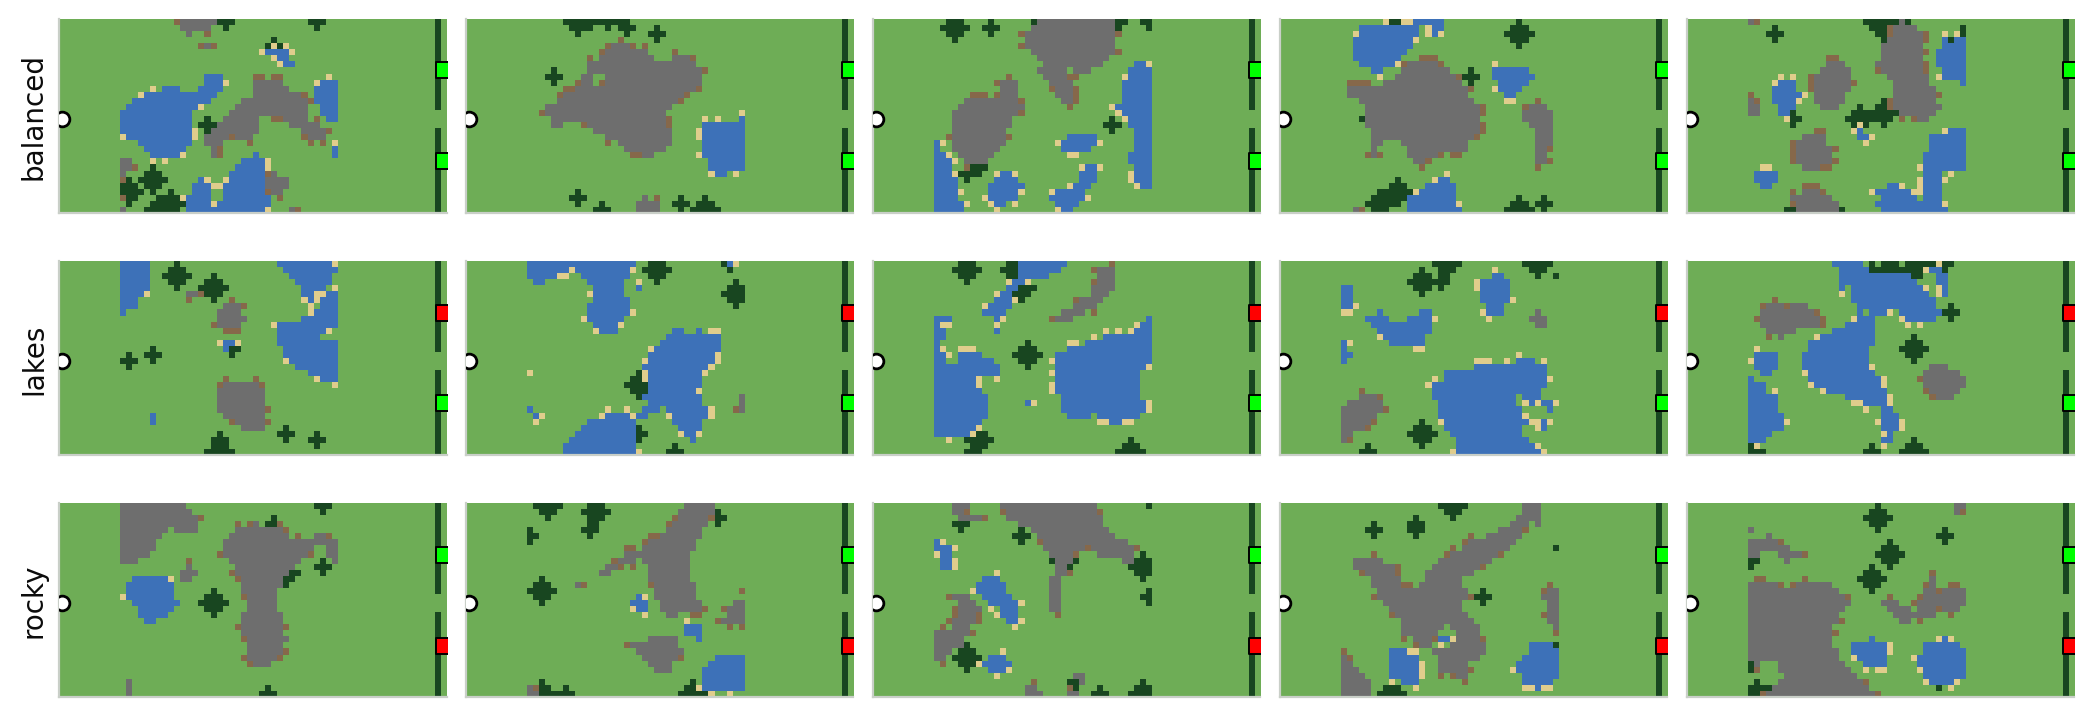
\includegraphics[width=\linewidth]{figures/fig_dataset_maps.png}
\caption{\textbf{Held-out maps by category}, five per row. Rows: balanced,
lakes, rocky. The white dot is the spawn, the green square the rewarding flag
and the red square the flag that pays nothing; on balanced maps both are
green. The three categories share one generator and differ only in the water
and rock quantiles, so no single tile identifies the category: it must be
integrated from the terrain seen along the way.}
\label{fig:dataset}
\end{figure}
